
%%%%%%%%%%%%%%%%%%%%%%%%%%%%%%%%%%%%%%%%%%%%%%%%%%%%%%%%%%%%%%%%%%%%
%%%%%%%%%%%%%%%%%%%%%%%%%%%%%%%%%%%%%%%%%%%%%%%%%%%%%%%%%%%%%%%%%%%%
%\definecolor{charcoal}{rgb}{0.21, 0.27, 0.31}
\definecolor{charcoal}{gray}{0.30}
\lstdefinestyle{console}
{language=bash,
basicstyle=\scriptsize\ttfamily\color{white}\bfseries,
backgroundcolor=\color{charcoal},
keywordstyle=\color{white},
alsoletter={:~$},
}


\chapter{Administration}


% ==================================================================
\section{Users, Groups and Authorizations}

% -----------------------------------------------------------------
\subsection{Overview}

\webobs uses its own AUTHORIZATION system, in addition to the Apache Authentication system, to identify its HTTP USERS and
control their individual ACCESS-RIGHTS to \webobs RESOURCES (ie. logical entities refering to files, processes, html-pages, whatever). 

AUTHORIZATION system elements:
\begin{itemize}
\item    a USERS TABLE that further identifies the USERS defined in the Apache Authentication files (eg. .htpasswd),
\item    a GROUPS TABLE that merely defines groups of USERS, to simplify (reduce number of) access-rights definitions,     
\item    RESOURCES are fully identified as \textbf{resourceType.resourceName}, 
\item    RESOURCES TABLES are the \textbf{resourceType} tables containing their own \textbf{resourceName} descriptions, 
\item    a \textbf{resourceName} description defines the relationship \textbf{uid-or-gid has access-rights},
\item    Supported access-rights are:
\begin{itemize}
\item    \textbf{R} = 1  Read 
\item    \textbf{E} = 2  Edit = Read + Write
\item    \textbf{A} = 4  Admin = Edit + Create/Delete
\end{itemize}
\end{itemize}


% -----------------------------------------------------------------
\subsection{Users table and Groups table}
\label{usertable}

A \webobs USER is identified by its LOGIN (string) as also defined in the HTTP Authentication system. A row in  
the USERS TABLE further defines a USER with the following information: 

\begin{itemize}
\item   LOGIN
\item   FULLNAME, the user's name
\item   UID, a short identification string, usually the user's name initials, to be used for access-rights and other functionnal needs
\item   EMAIL, the email address (somebody@somewhere) used by the \webobs POSTBOARD system,
\end{itemize}

Two special UIDs are reserved for system use: 
\begin{itemize}
\item   \textbf{?} to identify a GUEST user (granted to undefined users for temporary/limited access to \webobs), 
\item   \textbf{!} to identify the WEBOBS OWNER.
\end{itemize}

Records of the GROUPS TABLE associate UIDs to GROUP names (aka GID). A GID must starts with a '+' sign.
A USER may be a member of more than one GROUP. A USER inherits all access-rights defined for the GROUP(s) it belongs to. 

Four (4) special GROUPs are pre-defined in \webobs: \textbf{+ADMIN}, \textbf{+DUTY}, \textbf{+OBSERVER} and \textbf{+VISITOR}. They are initially used to  
define access-rights to \webobs built-in tools and/or applications. 

% -----------------------------------------------------------------
\subsection{Resource tables}

The fully qualified name of a \webobs RESOURCE is \textbf{resourceType.resourceName}.

There are five (5) resourceType tables: \textbf{authviews}, \textbf{authprocs}, \textbf{authforms}, \textbf{authwikis} corresponding to the base \webobs objects 
and \textbf{authmisc} for any additional, unclassified, resourceNames definitions. They are already populated with resourceNames related to \webobs built-in tools and applications.

The special resourceName "\textbf{*}" stands for "all resourceNames of this resourceType".

resourceNames are strings, defined and documented by the developers of the \webobs tools or applications.

% -----------------------------------------------------------------
\subsection{Managing Users and Authorizations}

The USERS ADMIN page \textbf{/cgi-bin/usersMgr.pl} (built-in tool), initially restricted to the +ADMIN group, is used to create/modify/delete user and resources definitions.

USERS and RESOURCE TABLES have customization variables in the main configuration file \wofile{WEBOBS.rc}:

\begin{lstlisting}[title=\wofile{WEBOBS.rc} (excerpt)]
SQL_DB_USERS|${ROOT_CONF}/WEBOBSUSERS.db
SQL_TABLE_USERS|users
SQL_TABLE_AUTHPROCS|authprocs
SQL_TABLE_AUTHVIEWS|authviews
SQL_TABLE_AUTHFORMS|authforms
SQL_TABLE_AUTHWIKIS|authwikis
SQL_TABLE_AUTHMISC|authmisc
SQL_TABLE_GROUPS|groups
\end{lstlisting}

% -----------------------------------------------------------------
\subsection{Developing with Users and Authorizations system}

The \textbf{WebObs::Users} perl module is the built-in interface to the USERS/AUTHORIZATIONS objects and functions system.
Detailed programming information can be found in its 'perldoc' documentation, such as:

\begin{itemize}
\item   global variables USERS, USERIDS and CLIENT
\item   the special 'path-like' specification for resourceNames
\item   functions: \textbf{allUsers, clientHasRead, clientHasEdit, clientHasAdm, listRNames}
\end{itemize}

Developers may add/define/use their own resourceName(s) for their specific needs.


% -----------------------------------------------------------------
\subsection{Adding a new user}

Registration of a new user is done in 3 steps:

\begin{enumerate}
\item new user must fill the form (see screenshot \ref{regform}) by connecting to WebObs interface and click 'Cancel' when asked to login. The data (with encrypted password) will be stored as a new pipe-separated line in the file \wofile{DATA/DB/reglog} and an e-mail will be sent to user and \webobs owner;
\item using Users Admin interface, administrator adds the user (see section \ref{usertable});
\item add manually the encrypted password as a new line to the file \wofile{CONF/htpasswd}; this activates the Apache user.
\end{enumerate}


\begin{figure}
\center
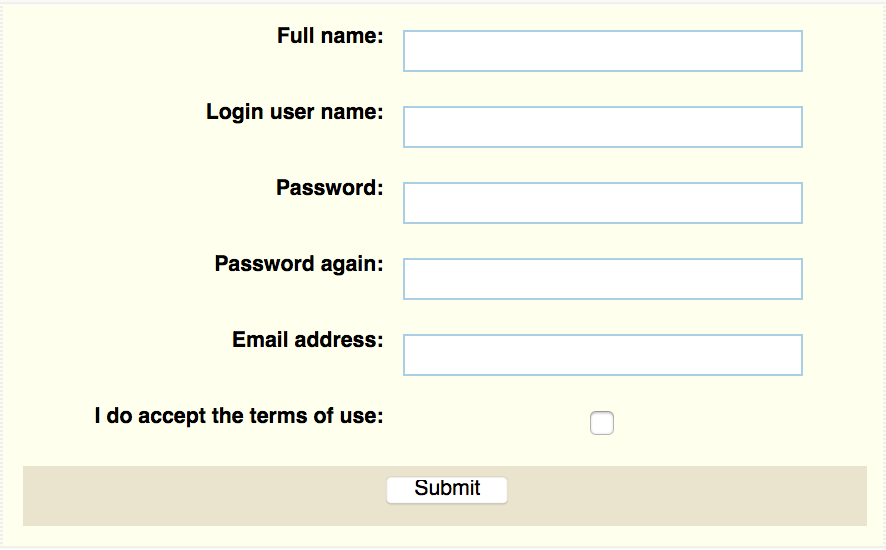
\includegraphics[width=.5\textwidth]{figures/registration_form.png}
\caption{Registration form for new users.}
\label{regform}
\end{figure}


% ==================================================================
\section{PostBoard}

% -----------------------------------------------------------------
\subsection{Overview}

\webobs tools and applications may wish to send (email) alerting/warning/information messages to \webobs USERs when detecting 
special processing conditions or other events. Deciding who needs/wishes to receive such messages, and actually sending them, should be
as easy as possible from the developers point of view; furthermore, \webobs administrators should be able to easily filter/choose which users 
should receive what, based on operationnal needs, authorizations concerns, and even user's choice of being (or not being) alerted.

The \webobs POSTBOARD system (notifications/subscriptions) addresses these needs. Elements of POSTBOARD architecture: 

\begin{itemize}
\item   Tools and applications simply and unconditionnaly send identified messages (NOTIFICATIONS) to POSTBOARD
\item   NOTIFICATIONS basically look like "eventname\textbar senderId\textbar message" 
\item   POSTBOARD is a daemon that tries to match the eventname of the NOTIFICATIONS it receives against active SUBSCRIPTIONS that 
tell it what to do: either send a mail to a UID (or GID), or trigger a command, or both
\item   a SUBSCRIPTION is a row in the \webobs NOTIFICATIONS TABLE with the following fields:

\begin{tabular}{ll}
\textbf{eventname} & identifying the SUBSCRIPTION to match NOTIFICATIONS sent to POSTBOARD\\ 
\textbf{validity}  & indicating active/inactive              \\  
\textbf{uid}       & UID or GID to whom mail the NOTIFICATION\\
\textbf{subject}   & subject of the mail being sent          \\  
\textbf{attachment}& optional, path of a file to attach to mail \\
\textbf{action}    & optional, a command to be executed      \\  
\end{tabular}
\end{itemize}

% -----------------------------------------------------------------
\subsection{Event names}

Event names identify and associate NOTIFICATIONS to SUBSCRIPTIONS:  
\begin{itemize}
\item   eventname    = string[.[string]] 
\item   string.string is known as the \textbf{majorname.minorname} form of an event-name
\item   \textbf{majorname.minorname} identifies a single subscription named majorname.minorname AND  
\item   a \textbf{majorname.} subscription, if defined as such (don't forget the ending dot!), will also match all \textbf{majorname.minorname} notifications
This is the way to define common mail/action to a set of notifications.
\item   some eventnames are already defined for internal \webobs usage. These reserved eventnames are :
\textbf{eventnode , formreq. , scheduler.alert , scheduler.warning , submitrc. }
\end{itemize}

Example: a \webobs application may issue (notify) NOTIFICATIONs identified with \textbf{myevent} eventname;  
The SUBSCRIPTION \textbf{myevent,Y,UID,mysubject,-,-} is registered in the NOTIFICATION TABLE; the following mail will 
eventually be sent by POSTBOARD when the application notifies "myevent\textbar \textbar the application message" : 

\begin{lstlisting}[title=mail for myevent notification]
From: webobs@webobsaddr
To: UID's mailaddr
Subject: [WEBOBS_ID] mysubject
User-Agent: Mutt/1.x.xx (2000-01-01)
the application message 
\end{lstlisting}


% -----------------------------------------------------------------
\subsection{Managing PostBoard Subscriptions}

The USERS ADMIN page \textbf{/cgi-bin/usersMgr.pl} (built-in tool), initially restricted to the +ADMIN group, is used to create/modify/delete  
the POSTBOARD SUBSCRIPTIONs in the NOTIFICATIONS TABLE.

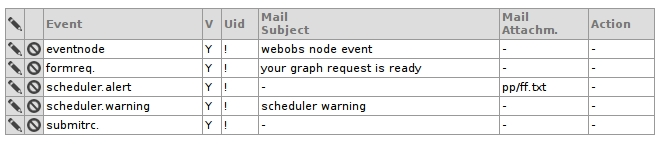
\includegraphics[width=.8\textwidth]{figures/subscriptions.png}

\textbf{CODE/cgi-bin/postboard.pl} is the Perl daemon.\\ 
\textbf{CODE/shells/postboard} is the command line interface 
to start/stop, query status and even send NOTIFICATIONs to POSTBOARD. 
Usage: \textbf{postboard [start\textbar stop\textbar status\textbar kill\textbar notify] }

POSTBOARD also has customization variables in the main configuration file \wofile{WEBOBS.rc}:

\begin{lstlisting}[title=\wofile{WEBOBS.rc} (excerpt)]
SQL_DB_POSTBOARD|${SQL_DB_USERS}
SQL_TABLE_NOTIFICATIONS|notifications
POSTBOARD_NPIPE|/tmp/WEBOBSNP
POSTBOARD_MAILER|mutt
POSTBOARD_MAILER_OPTS|-nx
POSTBOARD_MAILER_DEFSUBJECT|WebObs notification
\end{lstlisting}

% -----------------------------------------------------------------
\subsection{Developing with Notifications}

The \textbf{WebObs::Config} perl module exports the \textbf{notify} function to be used to send NOTIFICATIONS to POSTBOARD.
The \textbf{notify.m} module plays the same role from MatLab code. 

Detailed programming information can be found in \textbf{CODE/cgi-bin/postboard.pl} perldoc documentation, such as:

\begin{itemize}
\item   the \textbf{WebObs::Config::notify} function syntax,
\item   eventnames naming conventions,
\item   notification string syntax: \textbf{event-name}\textbar\textbf{sender-id}\textbar\textbf{message} and automatic timestamp ,
\item   \textbf{message} component interpretation and special keywords, 
\item   the special \textbf{submitrc.} eventname,
\item   POSTBOARD MAILER considerations,
\item   subscription's ACTIONs considerations
\end{itemize}


% ==================================================================
\section{Scheduler}
\label{scheduler}

% -----------------------------------------------------------------
\subsection{Overview}

The SCHEDULER is the daemon that controls the execution of \webobs batch JOBS. It has been developed to meet the following needs that,
for some of them, would have been more difficult to tackle, or simply have required as much development, with a regular crontab architecture:

\begin{itemize}
\item   schedule execution of a jobs based on the elapsed time since their previous execution,
\item   manage parallel executions of jobs,
\item   implement a mutually exclusive locking mechanism between jobs execution,
\item   implement a simple checking of CPU load to accept or delay jobs execution,
\item   centralize and normalize the jobs definitions, also with run-time parameters substitutions,
\item   standard output and error archiving and consultation,
\item   centralize reporting/history with housekeeping and HTML interface,
\item   accept dynamic jobs submission in addition to regular jobs,
\item   use \webobs POSTBOARD for errors/warnings and end-of-jobs notifications,
\item   provide both command line and HTML interfaces to JOBS and EXECUTIONS management 
\end{itemize}

The SCHEDULER daemon is \textbf{CODE/cgi-bin/scheduler.pl} whose execution is controlled with the command line interface \textbf{CODE/shells/scheduler}.

% -----------------------------------------------------------------
\subsection{Configuration and Tables}

The main configuration file \wofile{WEBOBS.rc} holds the \textbf{CONF\_SCHEDULER} variable that points to the SCHEDULER's configuration file used to 
customize its execution environment. Default configuration file is \textbf{scheduler.rc} :

\begin{lstlisting}[title=\wofile{scheduler.rc}]
BEAT|2                                        # internal processing loop frequency in seconds
MAX_CHILDREN|10                               # maximum number of simultaneously started jobs
PORT|7761                                     # commands' interpreter udp port number
SOCKET_MAXLEN|1500;                           # commands' interpreter max command size 
SQL_DB_JOBS|$WEBOBS{ROOT_CONF}/WEBOBSJOBS.db  # sqlite database for JOBS and RUNS tables
DAYS_IN_RUN|30                                # number of days JOBS are kept in RUNS table
DITTO_LOG_MAX|500                             # controls repeating messages in log
DITTO_NTF_MAX|1000                            # controls repeating messages notified
CANCEL_SUBMIT|600                             # max seconds submitted JOBS wait in Queue
CLEANUP_RUNS|999,zombie                       # how to tag zombie RUNS (unknown end of job)
LOADAVG1_THRESHOLD|0.7                        # max 1-sec cpu load threshold to start JOBS 
LOADAVG5_THRESHOLD|0.7                        # max 5-sec cpu load "
LOADAVG15_THRESHOLD|0.7                       # max 15-sec cpu load "
LMISS_BIAS|10                                 # seconds to delay candidates on load-threshold
EMISS_BIAS|4                                  # seconds to delay candidates on enq busy 
PATH_STD|$WEBOBS{ROOT_LOGS}/jobslogs          # root path for all STDOUT and STDERR of JOBS
PATH_RES|$WEBOBS{ROOT_LOGS}/res               # directory to hold JOBS resources (locks)
\end{lstlisting}


\subsubsection{JOBS TABLE}

JOBS to be scheduled are uniquely identified with a JID and defined into the JOBS TABLE by the following fields:

\begin{tabular}{ll}
\wocmd{JID}            &  JOB's ID unique string \\
\wocmd{VALIDITY flag}  &  indicates wether JID is eligible for execution \\
\wocmd{RESOURCE name}  &  a string identifying a mutually exclusive jobs lock \\    
\wocmd{XEQ1, XEQ2 and XEQ3}  &  3 components of the actual command that is started for JOB's execution \\
\wocmd{INTERVAL}       &  required elapsed time (seconds) between two executions of the JOB \\
\wocmd{LOAD THRESHOLD} &  max CPU LOAD value to allow execution of the JOB \\
\wocmd{LOGS PATH}      &  path of the JOB's STDOUT and STDERR files \\
\wocmd{LAST START TIMESTAMP} & (not editable) \\
\end{tabular}

\subsubsection{RESOURCE syntax}
A RESOURCE is simply identified by its freely choosen name (a string not containing double-dash, ie --). It may also 
be a set of individual resources (a '+' separated list of names): all of these individual resources must 
be simultaneously free for the job to be executed.

\subsubsection{XEQ1, XEQ2, XEQ3 syntax}

XEQ1, XEQ2 and XEQ3 will be concatenated, in this order, to build the actual JOB command to be executed. Those fields have no special
meanings for execution, except XEQ2 for LOGPATH (see below), and only one is obviously required to build a valid command; but they may ease maintenance and lisibility. 

They all accept variables interpolation: ie. they may specify any number of variable names from the main configuration file \wofile{WEBOBS.rc}, 
coded as \textbf{\$WEBOBS\{variableName\}}. 

\subsubsection{JOBS LOGS PATHS syntax}

JOBs can redirect/build their own STDOUT and STDERR, however the following rules are implemented as a default behavior in the SCHEDULER:  
\begin{itemize} 
\item   All JOBS outputs as a whole will be placed into the common \textbf{\$SCHED\{PATH\_STD\}} directory,
\item   JOBs' specific LOGPATH definitions are relative to this common directory  
\end{itemize}

The following table shows \textbf{LOGPATH} syntax (left) and its full interpretation (right), where 
any subdirectories will be dynamically created if needed, and \textbf{pid} is the JOB's PID (ie. KID) :

\begin{tabular}{ll}
\wocmd{name}          &	\$SCHED\{PATH\_STD\}/name.std\{out,err\} \\
\wocmd{name/}         &	\$SCHED\{PATH\_STD\}/name/pid.std\{out,err\} \\
\wocmd{name/name/out} &	\$SCHED\{PATH\_STD\}/name/name/name/out.std\{out,err\} \\
(null)                &	\$SCHED\{PATH\_STD\}/pid.std\{out,err\} \\
\end{tabular}

The following two redirection rules apply to any one of the above syntaxes:

\begin{tabular}{ll}
\wocmd{\textgreater name}             &  (the default) overwrites previous file with same name \\
\wocmd{\textgreater\textgreater name} & appends to previous file with same name \\
\end{tabular}

The following TAGS are also available in the name(s) you supply for easier specification of unique log files: 

\begin{tabular}{ll}
\wocmd{\{TS\}}    & replaced with job's start-timestamp \\
\wocmd{\{RTNE\}}  &	replaced with job's XEQ2 string, with any blanks (spaces) chars changed to \_ underscores. \\
\end{tabular}

% -----------------------------------------------------------------
\subsection{Jobs selection and execution}

The SCHEDULER continously scan the JOBS TABLE to find CANDIDATES for execution: ie those VALID JOBS whose LAST RUN TIMESTAMP is now older than their INTERVAL.

JOBS may also be submitted for immediate execution from the command line, or from another application, regardless of 
their INTERVAL normal delay and of their VALIDITY flag. Submitted JOBS are automatically CANDIDATES and placed in a 
JOB REQUEST QUEUE (JOBRQ) where they can stay no more than \$SCHED\{CANCEL\_SUBMIT\} seconds.

The SCHEDULER then scans all CANDIDATES, starting with the JOBRQ, to actually start (execute) JOBS that fullfill their CPU LOAD THRESHOLD and RESOURCE (lock)
conditions. JOB execution's command is the concatenation of the JID's XEQ1, XEQ2 and XEQ3 strings, in this order, and with \$\{WEBOBS\} variables interpolation.
Started JOBS are placed into a RUNQ for monitoring and future end-of-job processing, and in the RUNS TABLE for reporting/history.

CANDIDATES that are not moved to the RUNQ because they don't fullfill their CPU LOAD THRESHOLD and RESOURCE (lock) conditions,
will automatically be candidates again on the next scheduler's beat; to avoid unnecessary overload and reporting, the scheduler may delay these jobs
from being candidates again by a small amount of seconds. Delay to be used are defined by \$SCHED\{LMISS\_BIAS\} for CPU LOAD THRESHOLD condition and 
\$SCHED\{LMISS\_BIAS\} for RESOURCE busy condition. Set these to 0 to disable delay. 

JOBS are started as independent, parallel processes, children of the SCHEDULER, in their own process group; from there on they are known as KIDS.   
The SCHEDULER doesn't forget its KIDS once it forked them ! It waits for their termination (non-blocking wait) to perform housekeeping and reporting
about execution (mainly unlocking RESOURCEs, saving return code and elapsed time to update the RUNS TABLE). 

The precision at which JOBS are scheduled/executed is \$SCHED\{BEAT\} seconds.

Scheduler's job RESOURCEs, used as a locking mechanism between scheduled jobs, may be shared with external processes: thus it is possible
to also synchronize execution of scheduler's jobs with non-scheduler machine's activities and/or conditions. 
The Scheduler's commands ENQ and DEQ are the unique scheduler's entry points to the locking mechanism.  

\subsubsection{Command line submit syntax}

\begin{itemize}
\item   JOBS may be submitted, for immediate execution, to the SCHEDULER using \textbf{CODE/shells/scheduler} and its \textbf{submit} command
\item   specifying the JOB comes in two flavors:
\begin{itemize}
\item   JID=\textless job's id from JOBS TABLE \textgreater ; Example: \textbf{scheduler submit JID=myjob}
\item   as a string defining the JOB, with the following comma-separated keywords:
\begin{itemize}
\item   \textbf{XEQ1: , XEQ2: and XEQ3:} to specify the JOB's command
\item   \textbf{LOGPATH:} optional, to specify the directory, relative to \$SCHED\{PATH\_STD\}, for JOB's STDOUT and STDERR
\item   \textbf{RES:} optional, JOB's RESOURCE (lock)
\item   \textbf{MAXSYSLOAD:} optional, CPU LOAD THRESHOLD
\item   \textbf{UID:} optional, UID to be used for end-of-job notification
\end{itemize}
\item   Example:  \textbf{scheduler submit 'XEQ1:perl,XEQ2:/path/to/jobtst.pl,RES:mylock,UID:DL'}
\end{itemize}
\end{itemize}

Note: submitted JOBs are given a unique, negative, JID. 

% -----------------------------------------------------------------
\subsection{Scheduler manager}

The SCHEDULER MANAGER \textbf{CODE/cgi-bin/schedulerMgr.pl} built-in page, initially restricted to the +ADMIN group, is used to create/modify/delete JOBS of the JOBS TABLE. 

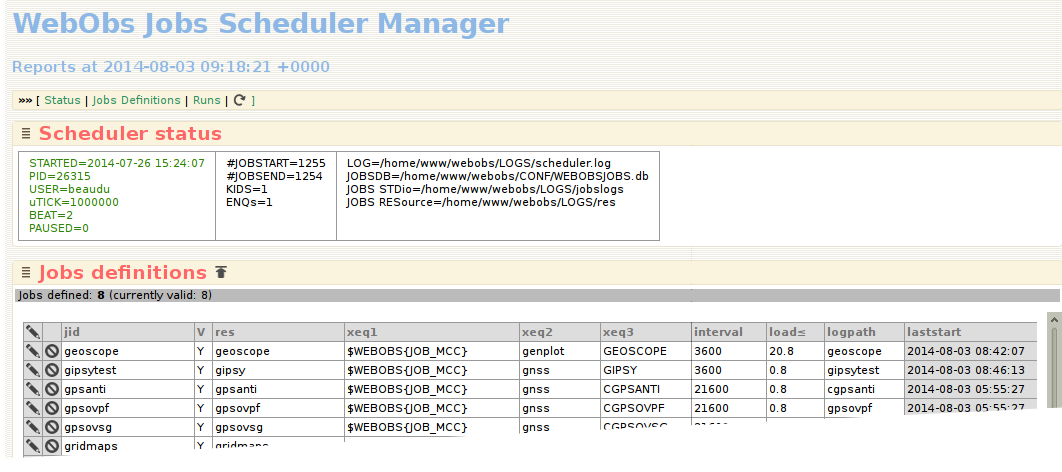
\includegraphics[width=\textwidth]{figures/schedmgr.png}

% -----------------------------------------------------------------
\subsection{Scheduler runs}

The SCHEDULER RUNS \textbf{CODE/cgi-bin/schedulerRuns.pl} built-in page, 
initially restricted to the +ADMIN group, is used to display the RUNS TABLE (one day at a time) along with its  
corresponding, zoomable TIMELINE chart, to better visualize JOBs executions elapsed times and parallelism. 

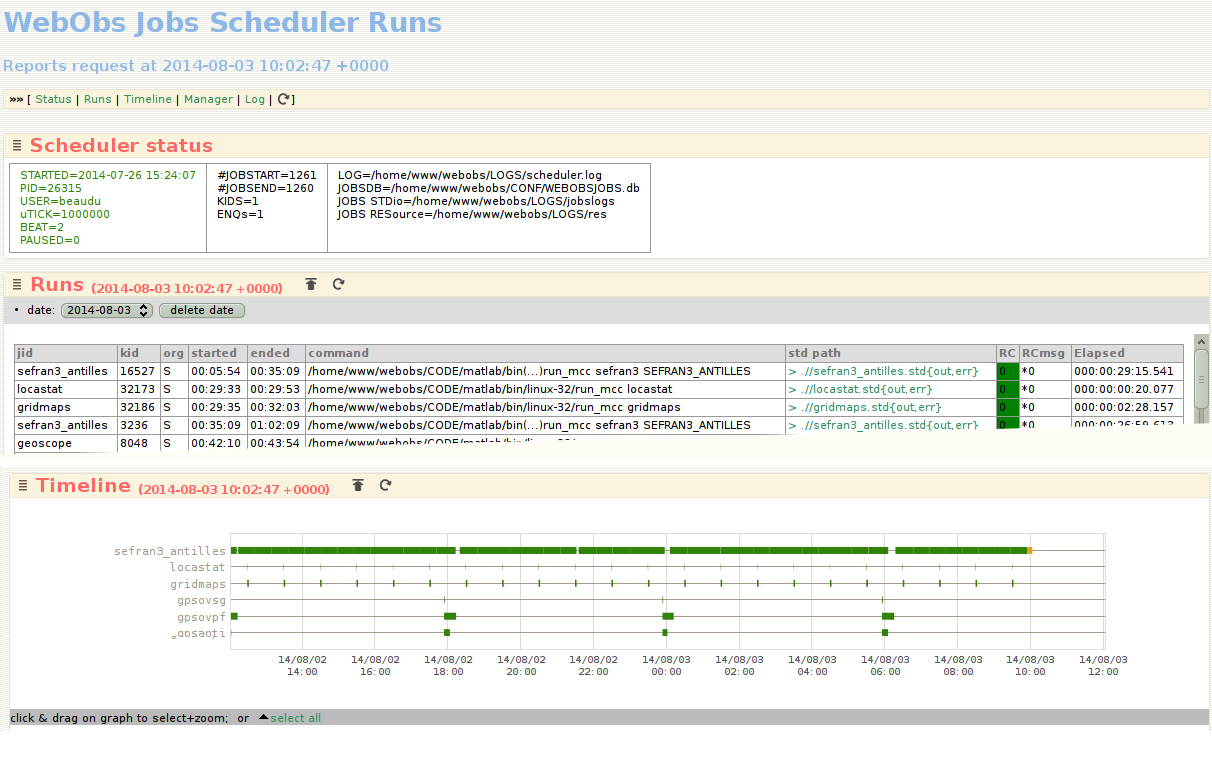
\includegraphics[width=\textwidth]{figures/schedrun.png}

% -----------------------------------------------------------------
\subsection{Scheduler status}

Both the SCHEDULER MANAGER and SCHEDULER RUNS built-in pages show the STATUS of the SCHEDULER:

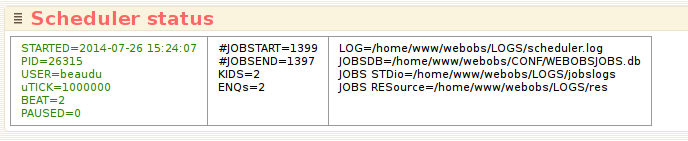
\includegraphics[width=\textwidth]{figures/schedst.png}

where:

\begin{tabular}{ll}
\wocmd{STARTED, PID, USER}  & \wocmd{when}, under \wocmd{which} PID and \wocmd{who} started the SCHEDULER\\
\wocmd{uTICK, BEAT}         & internal frequency in microseconds and main SCHEDULER loop frequency\\
\wocmd{PAUSED}              & wether SCHEDULER is in PAUSE mode (not scanning JOBs, = 1)\\
\wocmd{\#JOBSTART, \#JOBSEND} & number of \wocmd{started} and \wocmd{ended} JOBs since 'STARTED'\\
\wocmd{KIDS}                & number of currently started JOBs (KIDS)\\
\wocmd{ENQs}                & number of currently held JOBs' RESOURCEs\\ 
\wocmd{Paths} of main SCHEDULER's files & \\
\end{tabular}

% -----------------------------------------------------------------
\subsection{Scheduler command line}

The SCHEDULER command line interface is \textbf{CODE/shells/scheduler}. 

\begin{lstlisting}[style=console,title=shells/scheduler]
me@here:/opt/webobs/CODE/shells$ ./scheduler
Usage: ./scheduler {enq|deq|flog|jobq|kill|pause|ps|qs|quiet|resume|runq|start|status|stop|submit|verbose}
\end{lstlisting}

\textbf{CODE/shells/scheduler} sub-commands :

\begin{tabular}{ll}
\wocmd{start}    &   start, if not already active                       \\
\wocmd{stop}     &   stop, waiting for any active kids to end           \\   
\wocmd{pause}    &   hold execution (suspend jobs processing)           \\   
\wocmd{resume}   &   resume execution                                   \\   
\wocmd{enq}      &   enq a resource                                     \\   
\wocmd{deq}      &   deq a resource                                     \\   
\wocmd{kill}     &   forced stop, not recommended                       \\   
\wocmd{verbose}  &   log verbosity on                                   \\   
\wocmd{quiet}    &   log verbosity off                                  \\   
\wocmd{status}   &   display status/indicators/settings                 \\   
\wocmd{jobq}     &   display JOBRQ                                      \\   
\wocmd{runq}     &   display RUNQ                                       \\   
\wocmd{ps}       &   display executing KIDS trees                       \\   
\wocmd{flog}     &   force log backup and cleanup                       \\   
\wocmd{submit}   &   place a job on the JOBRQ, requiring additional arguments, either:\\   
                 &   1) \wocmd{jid=n}   where n is the JOB's ID from the JOBS TABLE \\
                 &   2) \wocmd{keyword:value[,keyword:value,...]} where \\
                 &      keyword in [XEQ1,XEQ2,XEQ3,MAXSYSLOAD,LOGPATH,RES,UID]
\end{tabular}

\begin{lstlisting}[style=console,title=example scheduler status]
me@here:/opt/webobs/CODE/shells$ ./scheduler status
Pls wait...
STATTIME=2014-02-05 06:04:58
STARTED=2014-02-05 06:04:02
PID=6725
USER=root
uTICK=1000000
BEAT=2
LOG=/opt/webobs/LOGS/scheduler.log
JOBSDB=/opt/webobs/CONF/WEBOBSJOBS.db
JOBS STDio=/opt/webobs/LOGS/jobslogs
JOBS RESource=/opt/webobs/LOGS/res
PAUSED=0
#JOBSTART=2
#JOBSEND=2
KIDS=0
ENQs=0
\end{lstlisting}

\begin{lstlisting}[style=console,title=example runq and ps]
me@here:/opt/webobs/CODE/shells$ ./scheduler runq
Pls wait...
RUNQ(1407212134.21663)
   kid=7567
   ORG=R
   uid=
   kidcmd=/opt/webobs/CODE/cgi-bin/jobtester.pl 40 
   res=
   jid=-2
   logfd=./
   started=1407212135.2194
   logfn=undef
RUNQ(1407211890.24512)
   kid=7060
   ORG=S
   uid=
   kidcmd=/opt/webobs/CODE/matlab/bin/linux-64/run_mcc sefran3 
   res=sefran3
   jid=sefran
   logfd=./
   started=1407211890.46864
   logfn=sefran3

me@here:/opt/webobs/CODE/shells$ ./scheduler ps
 PID  PGRP     ELAPSED %CPU %MEM CMD
2769  2769    02:41:40  0.0  0.1 /bin/bash
7050  7034       04:21  0.1  0.2 perl scheduler.pl -v
7060  7060       04:19  0.0  0.0   /bin/sh /opt/webobs/CODE/matlab/bin/linux-64/run_mcc sefran3
7068  7060       04:18  6.7  3.3     /opt/webobs/CODE/matlab/bin/linux-64/sefran3
7567  7567       00:14  0.0  0.0   /usr/bin/perl /opt/webobs/CODE/cgi-bin/jobtester.pl 40
\end{lstlisting}

% ==================================================================
\section{WOC}

\wocmd{WOC}, the \webobs \textbf{Console}, is a command-line tool to query and update internal \webobs structures.
Initially built as a developer's set of debugging tools and coding examples, \wocmd{WOC} also contains some \webobs administrator's tools. 

\wocmd{WOC} can be run in interactive mode, interpreting and executing woc-commands at the console's WOC prompt, or 
batch mode, executing a single woc-command passed as argument. \wocmd{WOC} is also available from a WebObs html page 
thru the use of woc.html + woc.js .

List of woc-commands :

\begin{longtable}{ll}
\wocmd{\%WEBOBS [key]}        &    dump \%WEBOBS key or all keys  \\
\wocmd{-\%WEBOBS value}       &    query which \%WEBOBS key(s) holds value  \\
\wocmd{\%OWNERS}              &    dump all \%OWNRS  \\
\wocmd{\%DISCP [discp]}       &    dump \%DISCP discp discipline or all  \\
\wocmd{\%USERS [login]}       &    dump \%USERS login or all  \\
\wocmd{authres}               &    list all  auth resources  \\
\wocmd{user login}            &    query DB USERS for login  \\
\wocmd{newuser}               &    add a user  \\
\wocmd{newgroup}              &    add a users group  \\
\wocmd{deluser}               &    delete a user  \\
\wocmd{delgroup}              &    delete a users group  \\
\wocmd{grant auth}            &    grant access in auth table  \\
\wocmd{auth login}            &    dump login authorizations  \\
\wocmd{\%NODES [key]}         &    dump \%NODES key or all  \\
\wocmd{proc [proc]}           &    dump PROC proc or all  \\
\wocmd{form [form]}           &    dump FORM form or all  \\
\wocmd{view [view]}           &    dump VIEW view or all  \\
\wocmd{node [node]}           &    dump NODE node or list node names  \\
\wocmd{newnode node as other} &    define a new node as othernode  \\
\wocmd{delnode node}          &    delete a node  \\
\wocmd{nodegrids [node]}      &    list grids that reference node  \\
\wocmd{nodedev [node]}        &    list features+devices for node (or all dev)  \\
\wocmd{statnodes}             &    statistics on node+grids  \\
\wocmd{readcfg file}          &    readCfg file  \\
\wocmd{dbjobs}                &    list all jobs definitions  \\
\wocmd{newjob}                &    add a job definition  \\
\wocmd{dbruns}                &    list all jobs last run info  \\
\wocmd{sys}                   &    print system information  \\
\wocmd{! cmd}                 &    exec shell cmd (WebObs vars single-quoted for interpolation)  \\
\wocmd{= expr}                &    exec perl expr (interactive mode only)  \\
\wocmd{dd}                    &    keys of main hashes and their occurence  \\
\wocmd{ddxref}                &    keys of main hashes + their occurence + cross-reference  \\
\wocmd{help}                  &    this help text  \\
\wocmd{quit}                  &    make a guess   \\
\end{longtable}


\begin{lstlisting}[style=console,title=WOC session example]

WOC version 1.6, Apr2013
At WOC prompt: command , 'help', or 'quit' 

<WOC> statnodes                                                                                                                                                                              
    14 node directories
     2 nodes have no grid
       GCSCC21  GCSREV1            
     0 node has no proc
     1 node has no view
       ISBFDF0              

<WOC> sys                                                                                                                                                                                    

Linux 3.2.0-67-generic #101-Ubuntu SMP Tue Jul 15 17:46:11 UTC 2014 GNU/Linux
Perl $^V = v5.14.2 
$ENV{PATH} = /usr/local/sbin:/usr/local/bin:/usr/sbin:/usr/bin:/sbin:/bin:/usr/games:
@INC : /opt/webobs/WebObs-beta-1.6.5/CODE/cgi-bin:/etc/perl:/usr/local/lib/perl/5.14.2:/usr/local/share/perl/5.14.2:/usr/lib/perl5:/usr/share/perl5:/usr/lib/perl/5.14:/usr/share/perl/5.14:/usr/local/lib/site_perl:.
$POSIX::VERSION = 1.24
POSIX::tzname = CET CEST
$ENV{TZ} = 
/etc/localtime -> CET-1CEST,M3.5.0,M10.5.0/3
local now: 2014-08-05 08:46:33 CEST (+0200) 1407221193 (1407221193)
UTC   now: 2014-08-05 06:46:33 1407217593 
$ENV{LANG} = en_US.UTF-8
Locale(s) Supported/Installed: en_US = S/I; fr_FR = S/I; 
UMASK 002
PID 12492 started 1407221193 by someone (1000/1000) in /opt/webobs/CONF


"WebObs-Paris" WebObs-beta-1.6.5 [/etc/webobs.d -> /opt/webobs/CONF]

<WOC> quit                                                                                                                                                                                   
Bye.
								 
\end{lstlisting}

% -----------------------------------------------------------------
\subsection{Overview}


